% !TeX encoding=utf8
% !TeX program = pdflatex
% !TeX spellcheck = en-US
% !BIB = biber

\documentclass[journal]{IEEEtran}
\ifCLASSINFOpdf
\usepackage[pdftex]{graphicx}
%\graphicspath{{./figs}{./moreFigures}}
\DeclareGraphicsExtensions{.pdf}

\usepackage{amsmath}
%\usepackage{algorithmic}
%\usepackage{array}

% Nice todo package based on tikz
\usepackage{todonotes}

% Nice references
\usepackage{cleveref}

% Shrink Itemize in table
\usepackage{enumitem}

%\usepackage[caption=false,font=footnotesize]{subfig}
%\usepackage{url}
\usepackage[acronym, shortcuts]{glossaries}

%\usepackage[backend=biber]{biblatex}
\usepackage{url}

\hyphenation{op-tical net-works semi-conduc-tor}
\usepackage{footnote}
%\setlength{\belowcaptionskip}{30pt}
%\setlength{\textfloatsep}{\baselineskip plus 0.2\baselineskip minus 0.2\baselineskip}
%\usepackage[belowskip=-15pt,aboveskip=0pt]{caption}

\usepackage{color}
% For highlighting changes in this version with red color
\newcommand{\highlighttext}[1] {\textcolor{blue}{#1}}
% Remove all text highlighting
% Useful to generate the final version of the PDF
%\newcommand{\highlighttext}[1] {#1}
\usepackage[belowskip=-10pt,aboveskip=5pt]{caption}
%\setlength{\intextsep}{10pt plus 2pt minus 2pt}

\makeatletter
\patchcmd{\@maketitle}
  {\addvspace{0.5\baselineskip}\egroup}
  {\addvspace{-1.2\baselineskip}\egroup}
  {}
  {}
\makeatother 
 
 
\usepackage{tabu}
 
\begin{document}
\title{Advancing Experimentation-as-a-Service \\Through Urban IoT Experiments}


\author{Dimitrios Amaxilatis,
        Dennis Boldt,
        Johnny Choque,
        Luis Diez, 
        Etienne Gandrille,
        Sokratis Kartakis, 
        Georgios Mylonas, 
        and Lasse Steenbock Vestergaard% <-this % stops a space
\thanks{The authors are listed in alphabetical order.}
\thanks{D. Amaxilatis and G. Mylonas are with Computer Technology Institute and Press Diophantus, Greece. E-mail:  \{amaxilat, mylonasg\}@cti.gr}% <-this % stops a space
\thanks{D. Boldt is with University of L\"ubeck, Germany. E-mail: boldt@itm.uni-luebeck.de}% <-this 
\thanks{J. Choque and L. Diez are with University of Cantabria, Spain. E-mail: \{jchoque, ldiez\}@tlmat.unican.es}
\thanks{E. Gandrille is with Commissariat \`a l'\'energie atomique et aux \'energies alternatives, France. E-mail: etienne.gandrille@cea.fr}
\thanks{S. Kartakis is with Intel Labs Europe, United Kingdom (E-mail: sokratis.kartakis@intel.com)}
\thanks{L. S. Vestergaard is with Alexandra Instituttet, Denmark. E-mail: lasse.vestergaard@alexandra.dk}% <-this 
}

%\markboth{Journal of \LaTeX\ Class Files,~Vol.~14, No.~8, August~2015}%
%{Shell \MakeLowercase{\textit{et al.}}: Bare Demo of IEEEtran.cls for IEEE Journals}
\maketitle

\begin{abstract}
Smart cities are becoming a vibrant application domain for a number of science fields. As such, service providers and stakeholders are beginning to integrate co-creation aspects into current implementations to shape the future smart city solutions. In this context, holistic solutions are required to test such aspects in real city-scale IoT deployments, considering the complex city ecosystems. In this work, we discuss OrganiCity's implementation of an Experimentation-as-a-Service framework, presenting a toolset that allows developing, deploying and evaluating smart city solutions in a one-stop shop manner. This is the first time such an integrated toolset is offered in the context of a large-scale IoT infrastructure, which spans across multiple European cities. We discuss the design and implementation of the toolset, presenting our view on what Experimentation-as-a-Service should provide, and how it is implemented. We present initial feedback from 25 experimenter teams that have utilized this toolset in the OrganiCity project, along with a discussion on two detailed actual use cases to validate our approach. Learnings from all experiments are discussed as well as architectural considerations for platform scaling. Our feedback from experimenters indicates that Experimentation-as-a-Service is a viable and useful approach.
\end{abstract}

\begin{IEEEkeywords}
Smart cities, Experimentation, IoT, real-world deployment, evaluation
\end{IEEEkeywords}

\IEEEpeerreviewmaketitle

% !TeX encoding=utf8
% !TeX spellcheck = en-US

\section{Introduction}
\label{sec:intro}

Information and Communication Technologies (ICT) are being adopted as a catalyst in the smart city domain, on top of which novel services are developed and legacy ones are evolved. In addition, the pervasive presence of ICT allows service providers and stakeholders to directly interact with citizens to continuously improve services in a co-creative manner. This co-creation approach permits the rapid deployment and adoption of innovative solutions for urban challenges~\cite{nasrawi}. A central part of instrumenting a smart-city with an IoT infrastructure is to be able to sense and monitor how the city performs, and to understand the dynamics of the city as a system. As examples, it becomes possible to examine how people make use of urban environments, and parameters like pollution, can be visualized and tracked throughout the city.

Recently, co-creation has been exploited in different ways by various \textit{Experimentation-as-a-Service} (EaaS) frameworks~\cite{vermesan2015building}. By ``co-creation'', we refer to the process of involving citizens and other stakeholders in designing as well as developing smart city solutions, and using local know-how to respond to existing challenges in modern cities and their communities.
For instance, Pallot and Pawar investigate co-creation to improve QoS~\cite{pallot}, while gamification techniques are used by Pokrić et al.~\cite{pokric}. Participation and interaction with stakeholders are used to attract people to the co-creation process~\cite{phuluwa, celino, gozard}. Finally, other work, such as Schaffers et al. ~\cite{schaffers2011}, focuses on technical aspects, in particular IoT or machine-to-machine communications, leaving aside user/citizen interaction.  In this sense, the scope of existing EaaS frameworks is limited to specific services or challenges. However, we believe that end-to-end solutions are necessary for harnessing the potential of complex city ecosystems. At the same time, the diversity in potential smart city applications makes it hard for a monolithic solution to satisfy their varied requirements. 

\begin{figure}
	\centering
	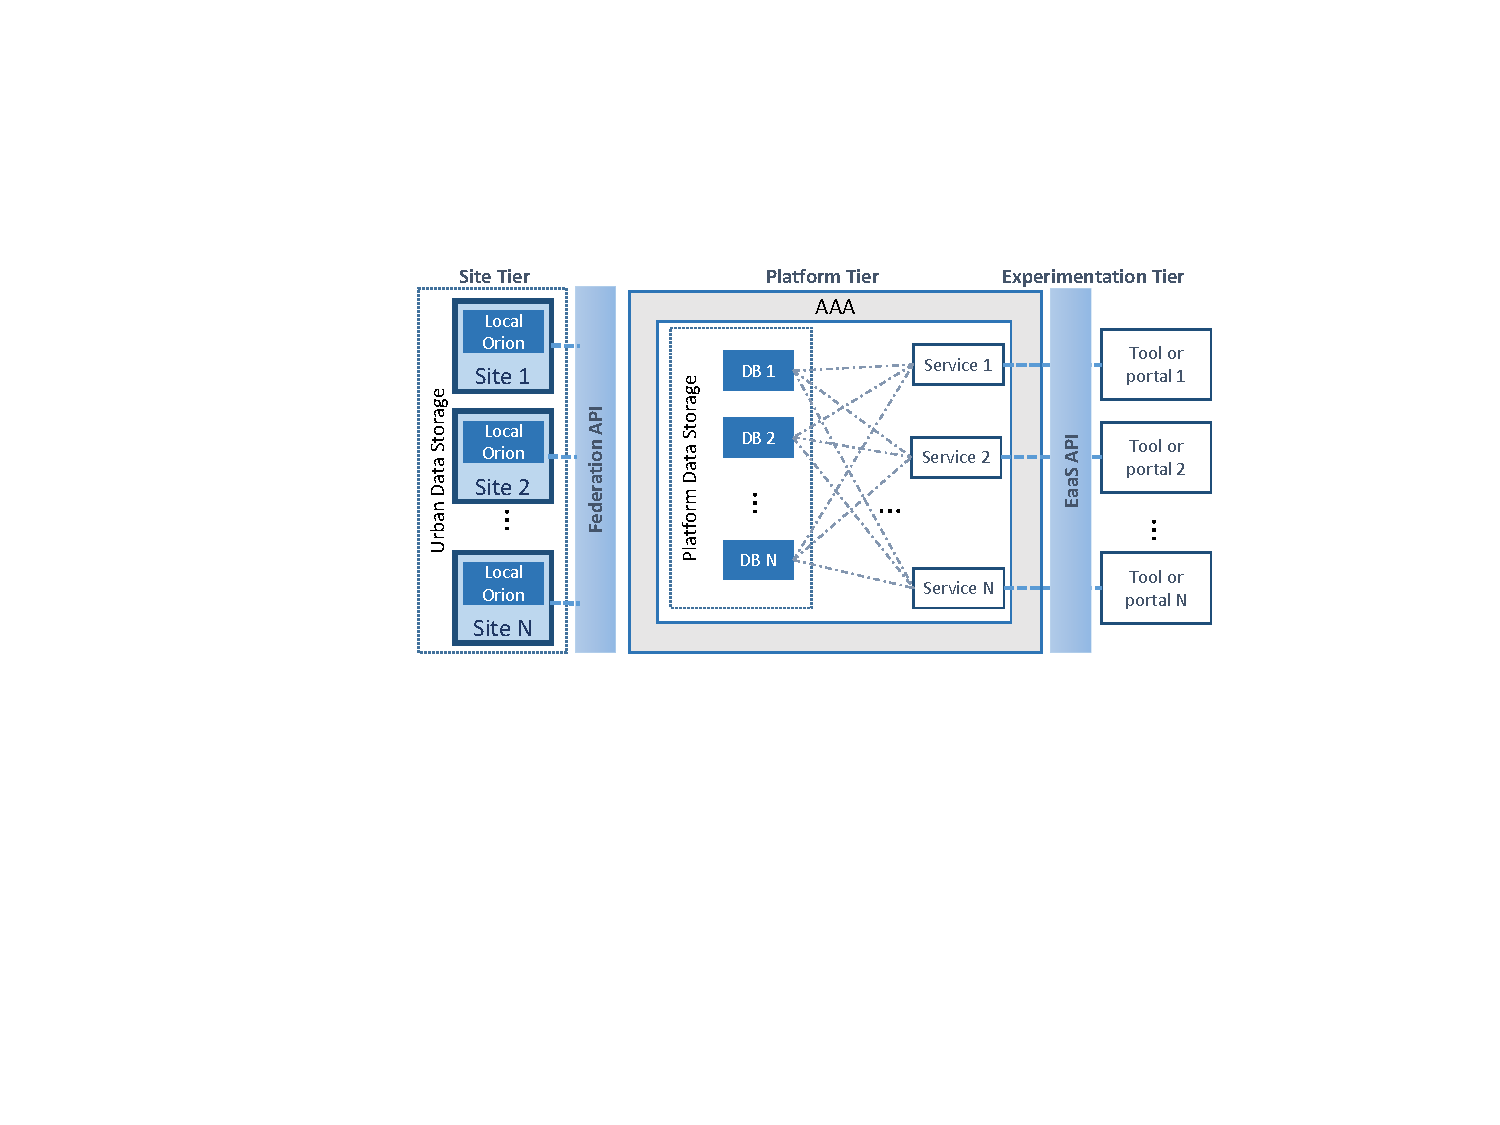
\includegraphics[scale = .66]{figures/simpleArchH}
	\caption{Overall OrganiCity platform architecture}
	\label{fig:arch}	
\end{figure}

In this context, the OrganiCity\footnote{OrganiCity H2020 project, http://organicity.eu} EU project (OC) developed a customizable EaaS framework, called the \emph{OC platform}. \highlighttext{The OC platform provides a common playground where different stakeholders can co-create urban services~\cite{gutierrez1}, and adopt the functionalities offered by the platform that better serve their needs}. As depicted in \Cref{fig:arch}, its design follows a three-tier approach~\cite{Schuldt2009}, addressing data provisioning, platform management, and experimentation support. It has been developed following an experimentally-driven approach, supported by \emph{open calls} during two periods (first open call in 2016--2017 and second open call in 2017--2018). \highlighttext{Open calls have had a twofold objective: first to help maturing the platform by gathering feedback from external users; and secondly to analyze the platform sustainability for the future.} \highlighttext{Throughout this paper, accepted open call projects are termed \emph{experiments}, and the actual people conducting these are referred to as \emph{experimenters} and \emph{experiment team} interchangeably. In addition, the term \emph{experimentation} refers to the process of conducting an actual experiment.}

\highlighttext{The first version of the OC platform~\cite{gutierrez1} was designed and validated within the OrganiCity consortium. This initial version was exploited during the first open call, which served to gather information and feedback from experimenters. Afterwards, the platform was tweaked according to the feedback and the new version was released in the second open call, which was devoted to developing a co-creation methodology for establishing cross-collaboration between stakeholders, communities, sectors and countries in a smart city context. In this paper we focus on the technical evolution, so that the work presented hereinafter spans from the period from which the OC platform was first deployed (initiation of first open call) to shortly before the second open call. In the first open call, a number of experiments have been selected and implemented, over a period of six months. Thanks to this key part of the OC project, experimenters have played an active role in the design and validation of our platform.}

In the following, we present a toolset to foster the development of urban services in a co-creative way. These novel services have been identified based on the feedback provided by 25 experiments conducted in five European cities (being from United Kingdom, Denmark, Spain, Greece, and Belgium), which have resulted in creating pilot services for more than 10 different urban application areas. In addition, the experiment teams involved different types of stakeholders, ranging from individual citizens to Small and Medium-sized Enterprises (SMEs), or public authorities. To our best knowledge, this is the first time that an EaaS framework is adopted in such a large scale manner, spanning over multiple cities. 

The rest of this work is structured as follows. First, \Cref{sec:sota} provides a discussion of related work, highlighting differences between existing approaches and ours. \highlighttext{Then, In \Cref{sec:lear}, the most relevant feedback obtained during OC platform exploitation, as well as possible modifications are explained. In \Cref{sec:adv} we describe the services developed after the first experimentation period, highlighting their functionalities and benefits.}  Finally, \Cref{sec:con} concludes the paper.
% !TeX encoding=utf8
% !TeX spellcheck = en-US

\section{Related Work}
\label{sec:sota}

In terms of experimentation testbeds, SmartSantander~\cite{sanchez2014smartsantander} built one of the largest city-scale IoT research infrastructures, pioneering the experimentation of novel smart city architectures, services, and applications in real-world urban environments. It emphasized managing experiments at an IoT device level, while allowing data-acquiring tasks facilitating urban services on top of the captured data flows. SmartSantander built interfaces with FIWARE and FI-Lab\footnote{https://lab.fiware.org}, to support interconnectivity with the IoT/Future Internet community. WISEBED~\cite{Coulson2012} pioneered discrete IoT device testbed federation. 

Additionally, projects like IoT-Lab\footnote{http://www.iotlab.eu} investigate crowdsourcing and IoT services for supporting multidisciplinary research tasks. Their approach differs from ours, since their services are not tightly coupled with a smart city testbed. Festival~\cite{Akiyama2017} is another example of existing federating experimentation testbeds from Europe and Japan, in order to provide a unified infrastructure to the research community. However, its focus is not exclusively on the smart city domain, and it does not offer the scale or the toolset provided by OC as a platform overall. CPaaS.io~\cite{FogFlow} is an ongoing project with similar goals to OC. Synchronicity\footnote{http://synchronicity-iot.eu} features open calls for developing new services, similar to OC, but places a much larger focus on open data markets in the context of a smart city, leaving aside the co-creative approach.

In light of these advancements, OC aims to combine the aforementioned approaches and co-create new smart city solutions with citizens, researchers and city authorities. Crowdsensing (i.e., tasking groups of volunteers to gather various kinds of data using IoT devices and/or smartphones) is one of the directions taken to address this challenge, helping to build a smart city data repository. Regarding the OC platform, a more general discussion is provided in~\cite{gutierrez1}, describing its architecture and overall software stack, with potential co-creation capabilities showcased in~\cite{gutierrez2} in detail. Apart from aiming to provide a pragmatic solution to the crowdsensing problem, the toolset discussed in this work allows end-users to benefit from this interoperability in various ways (data storage, visualization, interfacing to other systems, community management, knowledge extraction and urban service creation), and not just basic management of crowdsensing activities.

As an example of this approach, OC's crowdsensing tool allows for a broad set of opportunities for integrating smartphones in a smart city experimentation context, allowing the use of such devices to produce experimental data as an extension of an existing IoT infrastructure. %We allow for easy interconnection to other IoT devices, adding further possibilities to the system. 
The mobile crowdsensing paradigm and the associated features and challenges are further discussed in~\cite{%crowdsensing-guo, 
crowdsensing-guo2}. With respect to incentives and crowdsensing task assignment, which are also part of our work, in~\cite{aliens, incentives-survey} such aspects are discussed in detail. In addition, \cite{balestrini-orchestration, ledantec} provides a discussion related to several research questions we are trying to answer in OC as well. Finally, as discussed in \Cref{sec:intro}, OC has managed to appeal to a large number of research teams so far, and has already produced a large number of urban experiments, far surpassing the respective numbers kick-started by other similar projects.

% !TeX encoding=utf8
% !TeX spellcheck = en-US

\section{Learnings}
\label{sec:lear}

In this section, we discuss learnings from the initial deployment of the OC platform during the first open call. We shortly present two implemented experiments, and the experimentation teams' experiences from utilizing the OC platform. In continuation, we discuss the most common issues and comments experimenters have provided regarding their experiments. Finally, we discuss architectural considerations on how to robustly scale the OC platform in future deployments.

\subsection{Experimenter Experiences}

As mentioned in the introduction, 25 experiments were conducted in five different European cities during the first open call. All experiments used the OC platform, and each experiment team was required to report on their learnings with the OC platform. These reports were conducted twice: first through an interim standardized questionnaire, and then again at the end of the experiment. In this paper, we put emphasis on those inputs provided in the final questionnaires, since they bring richer descriptions of experiences with the technical part of the OC platform, than the interim questionnaires. In the following subsections, we present two specific experiments in order to show practical examples of how the OC platform has been utilized. We then discuss the most prevalent learnings reported by all experimenters.

\subsubsection{Spend Network}

 This experiment\footnote{https://organicity.eu/experiment/spend-network-2} aimed to develop a user-friendly, online based insight analysis tool for government, citizens and SMEs in London. The objective was to improve procurement efficiency and competition. The experimenters wanted to combine their own existing data with the OC platform in order to cross-reference with new data, and to perform enhanced spending and tendering categorizations. In order to make government spendings and tendering processes visible and easily understandable, the experiment used the TinkerSpace tool\footnote{https://docs.organicity.eu/tools/tinkerspace}, the Asset Federation API\footnote{https://docs.organicity.eu/api/Federation.html} and the OC's Urban Data Observatory (UDO)~\cite{gutierrez1}. TinkerSpace is one of the tools provided by the OC platform to simplify experiment development. This tool was used for the development of an interactive smartphone application where users are provided with an intuitive overview of the categorized data. The Asset Federation API was used for adding data to the OC platform in order to enable third party developers to use such data. Furthermore, adding data to the platform made it easier to connect them to TinkerSpace, thereby reducing development complexity. Finally, UDO was used for validating that assets were actually pushed to the OC platform, and for presenting them to third-party developers.

In general, the experimenters were satisfied with the OC platform, and managed to use the services, although not always as expected. They even developed new functionalities for the TinkerSpace tool, which they made publicly available for anyone to use. Despite of the good impression, they experienced several inconveniences with the OC platform. They reported that documentation was lacking or needed to be significantly improved for external developers to properly grasp and utilize the OC platform. Understanding the services, the documentation and getting support from the OC technical team required considerable waiting periods which they deemed inefficient resource usage. In addition to documentation, they reported that access to historical data was paramount for their experiment, and it was inconvenient that the OC platform did not provide such a feature at that time. They managed to solve the issue by providing a custom persistence feature. On top of these issues, the experiment team suggested that authentication on the OC platform should be more consistent, since they had to confirm their log in every time they navigated between different portals of OC.

Final comments from this experiment team revolved around maturity level of the platform in general. They reported that the UDO needed to further develop customization, TinkerSpace needed to significantly improve the usability, and the OC platform APIs were being re-factored during the experimentation period.

\subsubsection{WearAQ}

This experiment\footnote{https://organicity.eu/experiment/wear-aq-2} utilized IoT, machine learning (ML), wearable technologies, and citizen participation for investigating human perception of air quality in cities. This was done through developing gesture recognition gloves, worn by pupils during a walk around the city. The children were taught simple hand gestures that would signify whether they felt the air was polluted or not. In parallel, the experiment team did simultaneous air quality measurements with high-quality pollution monitoring equipment. The collected data was combined with data from the OC platform, and London air quality data assets. By applying ML techniques on the generated dataset, the experimenters identified that there was a correlation between the children's perception of air quality, and the measurements of the pollution monitoring equipment. 

In order to conduct the experiment, WearAQ utilized the Asset Federation API, Asset Discovery API, Scenario Tool and the UDO. The Scenario Tool was initially used, to get inspiration on how to shape their experiment. The UDO was used for searching environmental and traffic data within confined geographical areas. The Asset Discovery API was used for extracting real-time data for their ML models. Finally, they wanted to use the Asset Federation API for inserting their refined datasets into the OC platform, so that future experimenters can work with their findings.

Even though the experiment was successful, the team reported several issues with the OC platform. In their own words, ``there was a lot of documentation'', but they reported that parts of it were missing. There were inconsistencies between different documentation pages, some cross-referencing links were broken, and it could be hard to decipher the documentation from a non-technical perspective. They mentioned that it was difficult to grasp how to format parameters when using the RESTful APIs. They suggested that it might have been easier to comprehend if more usage examples were provided in the documentation. They also reported that error messages, returned from the APIs, were unclear. Apart from documentation issues, they reported that access to historical data was a lacking feature they had expected to be part of the OC platform, and they assumed that it was possible to manually upload assets directly through the Experimenter Portal. These missing features made the experiment more cumbersome, but they did mention that support from the OC technical team was good and swift, allowing the experiment to progress. \highlighttext{As a general comment, they stated that the OC platform felt a little shaky due to multiple platform updates during the experimentation period (in order to provide new features and bug fixing).}

\subsubsection{Overall Experimenter Learnings}

As mentioned previously, 25 experiments were conducted during OC's first open call. Through a grounded theory coding approach~\cite{charmaz2006constructing}, we conducted two iterations of analyzing the evaluation questionnaires. First, we performed an initial coding by annotating relevant passages with summative descriptions. In the second iteration, we conducted focused coding thereby abstracting the descriptions into nine overarching categories~\cite{charmaz2006constructing}. We have provided the categories in \Cref{tab:arch} (in alphabetic order), and further discuss these in the remainder of this section. A detailed usability assessment is available online in \cite{d55}.

From \Cref{tab:arch}, we see that the first deployment of the OC platform did not run smoothly, and this had consequences regarding how experimenters were able to use it in their experiments. Even though several issues and inconveniences occurred during the first experimentation period, the goal never was to have a fully fledged OC platform up and running from day one. Instead, we applied an experimentally-driven approach, where we wanted to collaboratively develop the OC platform with the experimenters. 

\begin{savenotes}
\begin{table*} 
	\centering
	\caption{Experimenter Experiences}
	\begin{tabular}{p{.1\textwidth}|p{.53\textwidth}|p{.3\textwidth}}\hline\hline
		\textbf{Category} & \textbf{Summarized experiences} & \textbf{Improvements}\\\hline
		
        Bugs & Reported bugs ranged from being inconsistencies in documentation (i.e., dead links) to not being able to create data assets through the Experimenter Portal, and experiencing that private assets where publicly available for third parties. Bugs could be small and insignificant to resulting in complete lock-down of developing an experiment. This means that bugs were present in all parts of the OC platform, and most experimenters experienced those at some point. & \highlighttext{Cleaning up documentation, fixing bugs, altering existing functionality and defining new services. User and Experiment management were services heavily refactored in order to fix bugs and provide a higher degree of management granularity (see \Cref{sec:adv}).}\\\hline
		
        {Data \hyphenation{Availability} Availability} & Data within the OC platform were outdated or not available when experimenters wanted to use them. The volume of data was too small, and it was challenging to find relevant data. & \highlighttext{Improved data search through an Annotations service and a Reputation service (see \Cref{sec:adv}).}\\\hline
        
		Documentation & This category has been heavily commented throughout all evaluations, and seems to be the pivot point for most of the frustrations during the experiments. We have divided this category into seven sub-categories (ordered alphabetically):
		
        %Shink the space on top and left of the itemize 
		%\begin{itemize}[topsep=-0.5cm,leftmargin=0.3cm]
        \begin{itemize}
			\item\emph{Ambiguity}: Ambiguous API naming conventions, abbreviations and contradictory documentation has been a hindrance.
			\item\emph{Error messages}: Vague, confusing, unhelpful and generic error messages were difficult to comprehend, and no documentation, on how to interpret the messages, was provided.
			\item\emph{Examples}: More and better usage and coding examples, as well as step-by-step tutorials are desired.
			\item\emph{Improvements}: Updating documentation more often, providing high-light examples, and use the Github\footnote{https://github.com} platform features even more would be of great value.
			\item\emph{Inconsistencies}: Parts of documentation was deprecated, had dead links, and errors like references to \emph{localhost} was not corrected. Documentation could suddenly change and there was inconsistencies between different documentation.
			\item \emph{Readability}: Documentation was not easy to comprehend for a non-technical person.
			\item \emph{Unclear descriptions}: Documentation was not sufficiently elaborated and hard to follow, it was not clear how to format API parameters and it could be hard to understand how the OC services should be used and interact.
		\end{itemize}%
        %\vspace*{2mm}%Hack to shrink the space below the itemize
		 & \highlighttext{Recognizing that documentation was the main source of frustration, this part has been totally refurbished. The new documentation\footnote{https://docs.organicity.eu/} first provides a general OC platform description for experimenters to become familiar with the modules and terminology. From such description, links are provided to different parts where technical information is provided. In addition, step-by-step tutorials have been elaborated covering the most relevant and recurring procedures. Finally, the APIs documentation has been reviewed to avoid inconsistencies.}\\\hline
         
		{{Lack of~} \hyphenation{functionality}functionality} & Two features were lacking, which experimenters had expected to be available. This is API access to historical data, and the ability to provide filtering options when searching for data. & \highlighttext{Historical REST-based data API introduced during first experimentation phase, and data filtering added to the UDO. WebSocket-based service developed for providing push notifications on asset updates (see \Cref{sec:adv}).}\\\hline
        
		Positive feedback & The OC platform was well designed and the available tools were both relevant and usable. Especially the graphical data searching (the UDO) was great for getting an overview of what data was accessible through the OC platform. One experiment team reported, that the authentication and authorization functionality enabled them to have a clear division between their own custom developed software and the OC services. & \highlighttext{Annotations and Reputation services added to the UDO. Improved ability to interface directly with the OC platform APIs. Particularly evident in the User management and Annotations services.}\\\hline
        
		Suggested new functionalities & Data visualization is quite simple in the OC platform, and is reduced to showing assets on a map in a browser. Experimenters would have liked more comprehensive data visualization features in order for them to play around with the data, and it could have simplified their custom developments. It was also reported that visualizations of historical data would have been beneficial. Finally, one experiment team reported that they wanted to have more fine grained authorization configurations in the APIs in order to control who could upload data to the OC platform. & \highlighttext{The UDO was continuously expanded, and a historical data graph was added at the very end of the first experimentation phase. Fine-grained user and experiment configuration have been added through the User and Experiment management services.}\\\hline
        
		Support & Level of support was satisfactory, and direct communication via phone, email or Slack\footnote{http://slack.com} was fast and helpful. A few experimenters reported that Slack could be confusing due to multiple channels, and occasionally response times were slow. & \highlighttext{Slack has been replaced by an open forum\footnote{https://docs.organicity.eu/}, based on the Q2A\footnote{http://www.question2answer.org/} platform, in order to reduce confusion and optimize support efforts.}\\\hline
        
		Technical breakdowns & The Experimenter Portal produced error messages, changes could not be saved and invitations to participants would not be sent. The OC platform crashed regularly initially, functionality was often refactored, and experimenters had to adapt their existing codebase. When adding new assets to the platform, errors would arise when API attributes contained special characters. & \highlighttext{Errors and issues were captured and major revisions carried out including: better functionality consistency, lower coupling between platform components, updating server infrastructure and architectural considerations.}\\\hline
        
		Usability & From a usability perspective, experimenters were divided. Half of the experimenters found the OC platform easy to understand and use, while the other half found it cumbersome and unnecessary complex. The latter consisted primarily of experiment teams with a non-technical background. Regarding the UDO, most experimenters found it easy to use and helpful for understanding the concept of the OC platform. On the other hand, most experimenters had difficulties understanding and using the authentication and authorization functionality. Parts of the issues came down to understanding OAuth2. & \highlighttext{A large part of the platform revisions have been pivoting around improving usability through step-by-step examples, expanding the graphical representation of User and Experiment management, reducing the steps needed to authorize against Keycloak, only expose relevant API functionalities etc.}\\
		\hline\hline
		
	\end{tabular}	
	\label{tab:arch}	
\end{table*}	
\end{savenotes}

As a result, the first deployment of the OC platform should be perceived as a prototype of how an EaaS framework could be composed. This also means that the OC platform, as a whole, was not user-tested until it was made available to experimenters. The experimenters were aware of that the OC platform was not fully functional, and they were consequently prepared for experiencing issues. Knowing that  experimenters would encounter problems, we set up several communication pipelines (e.g., email, Slack or phone) so that experimenters could easily get in contact, and thereby progress their own developments. When issues and bugs were reported, we did our best to fix them immediately, but we had to prioritize which were most critical. As a result, some bugs were not corrected during the first experimentation period, and we suggested workarounds instead. We made sure to plan the implementation of the reported features so they would be implemented after the first experimentation period (i.e., historical data storage). According to \Cref{tab:arch}, it seems that the provided support pipelines have been satisfactory. From an internal OC perspective, support took up significantly more time than initially expected.

After the first open call ended, we significantly improved the OC platform by adding new functionalities. We have provided API access to historical data, and documentation has been significantly re-factored with updated examples, step-by-step guides and tutorials. Dead links, due to the continuous updates in the platform's documentation, have been fixed and coherency between different documentation locations has been improved.

In relation to documentation, experimenters reported this to be the culprit of most of their technical frustrations. Despite this, an interesting finding is that several experimenters reported that reading documentation and debugging took too much time, which they felt was both wasted and insufficient. We do not have specific figures on how much time experimenters actually spent on these activities, but empirical studies and our own experiences show that professional developers usually spend around 70\,$\%$ of their development time doing nothing but reading documentation and debugging~\cite{Minelli2015}. The expressed frustration was therefore a result of the non-technical nature of the experimenters participating in the open call. Since we do not have metrics for comparing time spent on actual programming, it is not possible to measure the efficiency of the OC platform's documentation, but according to the experimenters, this part took up a significant amount of their development time. In hindsight, this indicates that high quality documentation is of utter importance when exposing an EaaS platform to third-party developers.

\subsection{Architectural Considerations for Platform Scaling}

As we have commented in Section~\ref{sec:intro}, OC followed a centralized data architecture for both, storing and search. However, this approach may have scalability constraints, and hinder its adoption. In this sense, the ETSI\footnote{http://www.etsi.org} has created the Context Information Management (CIM) group, which is actively working on evolving the current definition of OMA-NGSI~\cite{NGSIOMA} and Orion Context Broker~\cite{FiwareOrion}  implementation (referred to as Orion in the remainder of this paper), developed by the FIWARE EU Initiative\footnote{https://www.fiware.org}. The preliminary technical specification of the so called NGSI-LD has recently been published~\cite{NGSILD}, and it proposes different options to deploy centralized and distributed architectures. In the following, we describe the different options that can be adopted and how they fit with the existing OC platform. 

Since we have followed a centralized approach, the different OC services access the central Orion for any data related action. As mentioned, this yields scalability limitations, and enforces to having a centralized architecture. In order to overcome such limitations, we are studying how to use NGSI-LD functionalities to enable hierarchical and distributed context information storage. \Cref{fig:arch2} provides an overview of federation with distributed storage.

Similar to the current OC architecture presented in \Cref{fig:arch}, the future approach will consider that different sites (i.e., cities) produce data that can be federated with a central OC instance. Cities will host local instances of Orion, that will be fed by context producers. Typically, the producers are services run by city service providers, that generate information which the city stores. Then, the site brokers notify the context registry about the locally stored data. Different to the current OC implementation, the registry does not store the data, but only where the data can be found. Finally, a distribution broker acts as proxy to access the data, by checking the data location in the registry. As can be observed, in this approach no data duplicates are generated, thus solving scalability issues. In addition, it is possible to replicate the same architecture at different scales, as depicted in Figure~\ref{fig:arch2}. This way, a site broker can internally act as a distribution broker. Furthermore, this approach will also enable cities to deploy local instances of OC with the required micro-services, while still being part of a larger deployment.

\begin{figure}
	\centering
	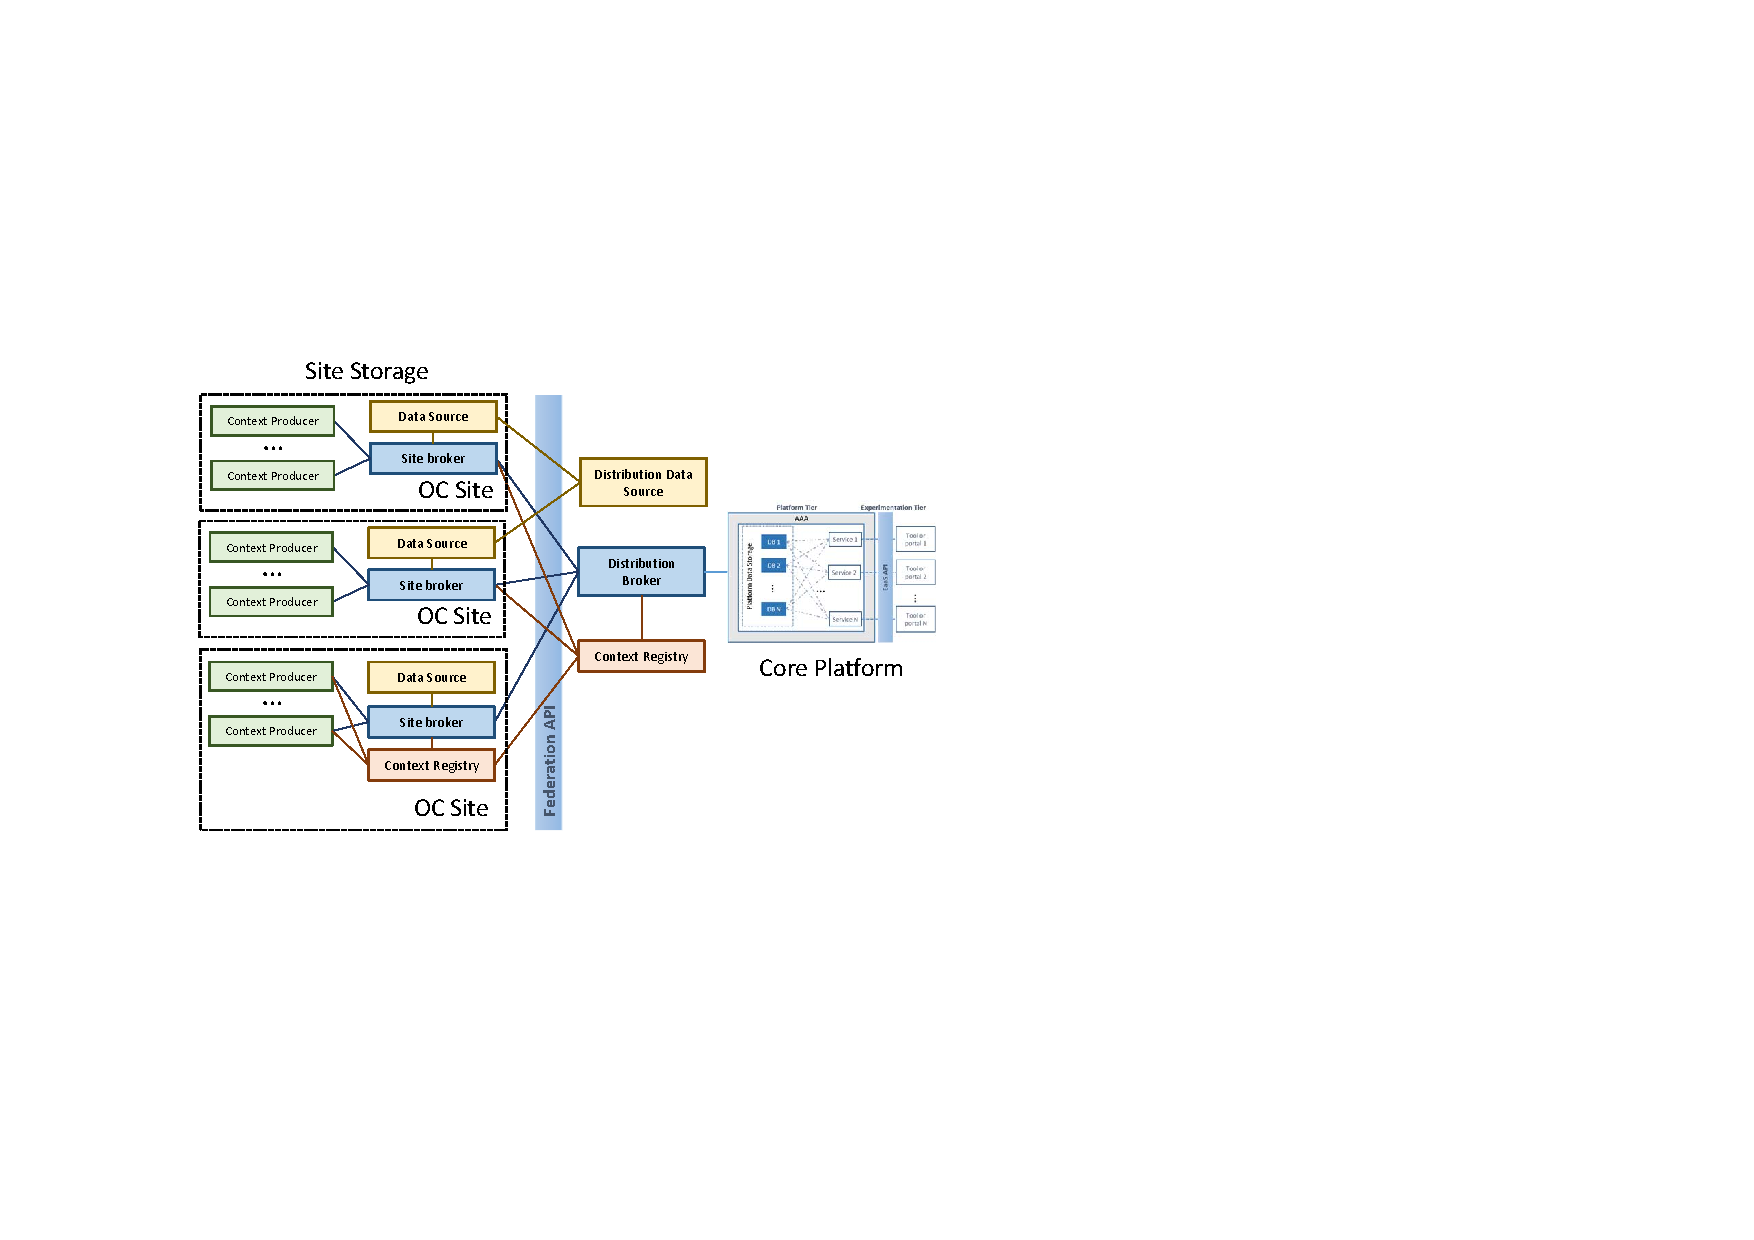
\includegraphics[width=\columnwidth]{figures/archExt}
	\caption{Distributed federation architecture}
	\label{fig:arch2}	
\end{figure}
% !TeX encoding=utf8
% !TeX spellcheck = en-US

\section{Advanced EaaS Services}
\label{sec:adv}

As depicted in \Cref{fig:arch}, the OC platform design follows a three-tier approach, addressing data provisioning, platform management, and experimentation support. The Site Tier accounts for the data sources (e.g., cities) federated in the OC platform (named OC site). The Platform Tier holds the platform services, which are exposed for experimentation in the Experimentation Tier. The persistence within the Platform Tier relies on Orion, which is  built around the NGSI~9/10 protocols. It manages entries, called assets, which can represent devices, places, buildings and any other context information entities (including virtual objects). Each asset holds a set of typed attributes which can be updated on the fly~\cite{gutierrez1}. The Platform Tier has been designed using loosely coupled and distributed components following the micro-service architecture pattern~\cite{newman2015building}. This allows tailored deployments involving only the mandatory, or baseline services, so that others (i.e., APIs, tools and portals) can be optionally deployed.

The rest of this section covers improvements performed in the Platform and Experimentation Tiers. This tier makes use of the EaaS APIs (see \Cref{fig:arch}), and it embraces tools and Web-based user interfaces (web portals). Each EaaS service (i.e., API, tool and portal) is implemented as a micro-service. In this sense, some of them are standalone applications, while others rely on baseline services, such as the Orion or the User Management. For a more detailed description of the platform, the reader may refer to ~\cite{gutierrez1}, which covers the EaaS services, which were used in the first open call. \highlighttext{Based on feedback from experimenters in the first open call, we re-factored and extended the OC services, and present these in the following sub-sections.}

\subsection{User Management}

Within OC, we cater to different stakeholder ``roles'', e.g., administrators, site managers, experimenters and participants. An administrator is the technical administrator of the OC platform and, therefore, has access to information of all experiments at platform level. A site manager manages an OC site, which is a set of assets under a common administrative domain available for experimentation, e.g., the assets of a city. Each role is allowed to access different systems, which consists of an API and a portal. To handle this, we developed a User Management system to handle authentication and authorization.

\begin{figure}
%	\todo[inline,author=Dennis]{Shall I create a blue version of the figure?}
    \centering 
	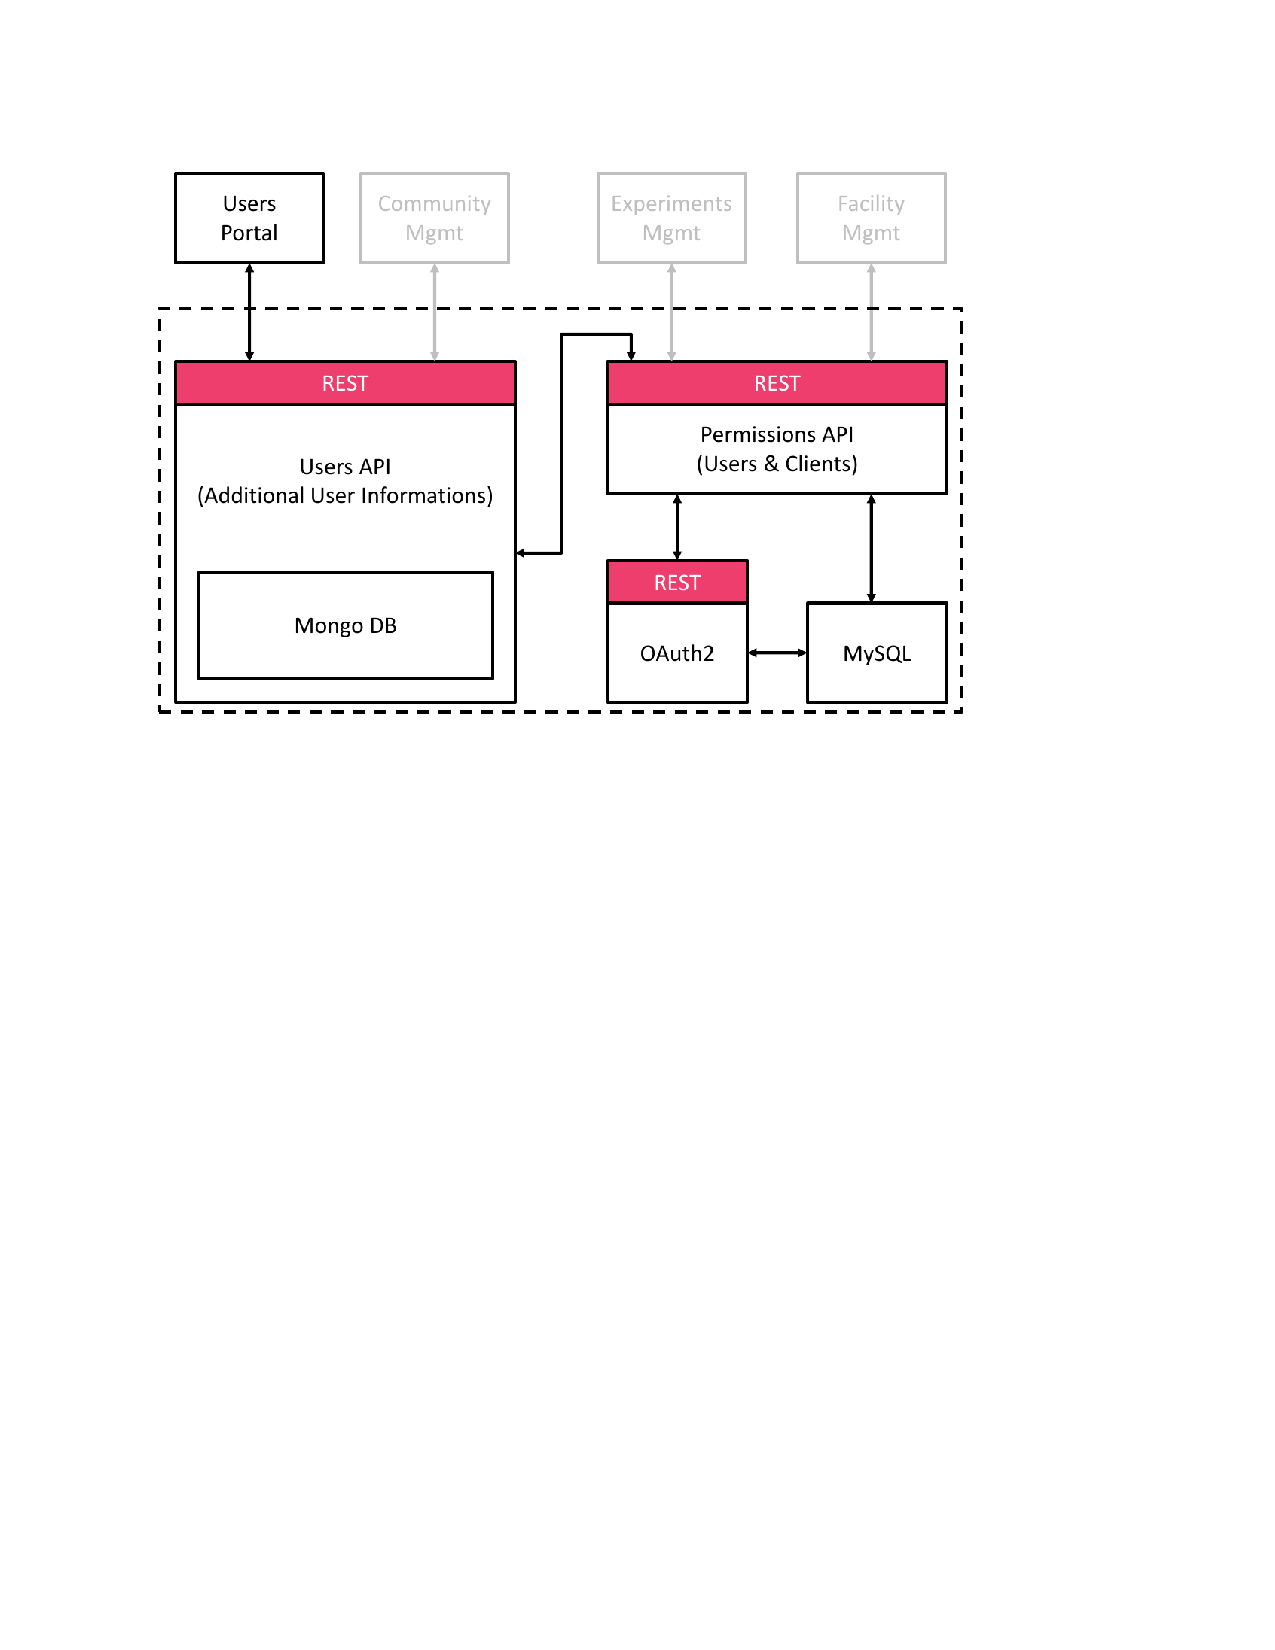
\includegraphics[scale = .5]{figures/user}
	\caption{User Management APIs}
	\label{fig:user}	
\end{figure}

The User Management API is based on OAuth2's API~\cite{rfc6749}, with a single sign-on service, a \emph{Users API}, and a \emph{Permissions API} (see \Cref{fig:user}). They are used to manage accounts for users and clients (e.g., OC services). We use KeyCloak\footnote{https://www.keycloak.org} as an OAuth2 server. %To manage accounts, it provides an HTTP-based RESTful API~\cite{fielding2000architectural}, which is only usable by KeyCloak-specific \emph{admin} accounts. 
To allow other OC services to manage accounts, we created the Permissions API, which acts as a configuration proxy for a more fine-grained access to the roles and permissions of accounts. Users must register at the server and verify their account by email. Afterwards, a user can log into all OC services by using a single account. %In case of the portals, a user needs to log in only once, since a session is used to remember the user. 

The \emph{Users Portal} allows users to manage their data, such as user and real names, nationality, email, age, etc. The Users API allows a quick and efficient user search for other OC services, since it uses MongoDB\footnote{https://www.mongodb.com}. Some information like the username, email and password is synced between the Users API and the KeyCloak server. Authentication and authorization are still handled by the OAuth2 API, the other OC services can use the Users API to manage accounts.

\subsection{Experiment Management}

One of the key aspects of the OC platform is the definition of an experimentation management system, able to fulfill the requirements of potentially heterogeneous experiments. This system has been implemented as a set of APIs exposed through three web portals. First, the \textit{Experimenter Portal} allows experimenters to manage all aspects related to experiment management and exploitation. Closely related, the \textit{Communities Portal} enables the grouping of users, based on their interests and preferences, into the so called communities. Finally, the \textit{Participant Portal} permits potential participants to manage the experiments in which they are enrolled. \highlighttext{We briefly describe the functionalities of each of the web portals in the following.}

\subsubsection{Participant Portal}

This portal is used by users registered in OC, who have stated their willingness to participate in experiments, and it offers three main functionalities:

\begin{itemize}
	\item\emph{Experiment search}: All public experiments are visible to the participants, they can proactively select those taking place close to them or that are considered interesting, according to the experiment information.
	\item\emph{Notifications}: Participants can be notified about any event happening in the experiments they are involved in, and they can be invited to new experiments. It is worth noting that all interactions happen in \textit{an anonymous way}. Experimenters are not aware of the identity of participants.
	\item\emph{Enrolling management}: Participants can decide to leave an experiment at any point. It is applied to both experiments, which they proactively joined, and those which they were invited in.
\end{itemize}

\subsubsection{Communities Portal}
 
Once users register in OC, they can complete their profile by providing more information about their interests and preferences. Through the Communities Portal, administrators and experimenters can filter users and create \emph{communities}. A community is a virtual group linked to an experimenter or administrator, in a way that users and participants are not aware of the communities they belong to. %In the same way, 
Moreover, experimenters and administrators are not aware of the actual identity of the user in their communities, but they see simple indicators on the characteristics of their community's audience.

\subsubsection{Experimenter Portal}

This portal is the entry point of experimenters to the OC platform, and serves as a hub for the experimentation services. Following the micro-service design of the entire OC platform, the Experimenter Portal incorporates new services as independent views which may eventually be deactivated depending on the actual requirements. \highlighttext{By using the Experimenter Portal, experimenters can perform the following tasks}:
%The main functionalities provided by the Experimenter Portal are related to the management of the experiment instance, and cover deployment and experimentation:

\begin{itemize}
	\item \emph{Creation and management of experiments}: This functionality utilizes the User Management API. \highlighttext{Following the dominant concept in IoT experimentation, each experiment instance is seen as a virtual testbed, and uniquely identified throughout the whole platform. This way experiment datasets and management information can be isolated. In addition, at any moment experiments can be stopped/restarted and edited (e.g., name, description, etc.)}. 
	\item \emph{Creation and management of assets}: Leveraging the public platform APIs, the Experimenter Portal provides a graphical UI to create and edit assets, in order for experimenters to become familiar with the data format. \highlighttext{In particular, the graphical UI is a JSON editor able to check that the data follows the OrganiCity format, providing useful warning messages otherwise.}
	\item \emph{Experiment team management}: \highlighttext{Since co-creative experiments usually involve development teams rather than a single person, the Experimenter Portal also permits editing such teams. In this regard, at any moment the creator of the experiment can edit the team by adding or removing their members.}
\end{itemize}	

Apart from the aforementioned functionalities, the Experimenter Portal also provides views closely related to other services, and that can be used by the experimenters.

\paragraph{Annotations}

The Experimenter Portal offers a UI to manage \emph{tags} that can be applied on the assets created under each experiment. Experimenters can both select tags provided by the OC platform itself, or define new ones, available only for their own experiment. Tags are explained in more detail in \Cref{sec:annotation-service}.

\paragraph{Participants Management and Engagement Monitoring}

By using the communities created with the Communities Portal, experimenters can invite people to their experiments, and check whether or not invitations have been accepted.
In addition, experimenters can define engagement metrics as a function taking into account different parameters. Then, during the execution of the experiment that function grows differently for the different participants according to the engagement level. For instance, a function can be defined as the amount of created data, number of readings or the number of annotations added by a participant. Finally, using the notification functionalities provided by the platform, experiments can reward or incentivize participants.

\subsection{Real-Time Notifications}

The requirement for real-time data is crucial for understanding and enhancing the smart city~\cite{jin2014information}, which is why the OC project has chosen to emphasize the need for real-time data streams when performing experiments through the OC platform. This is both relevant for city administrators needing to optimize and predict city infrastructures but also for ordinary citizens who want to understand and affect the city~\cite{jin2014information}. Real-time access to city data can even become a collaboration interface between city administrators and regular citizens in developing the city. A specific example of such a collaboration is the application \emph{Bus Santander}\footnote{http://bussantander.truebaj.com} that shows real-time estimates on when a bus arrives at a bus stop. The application was developed by ordinary Santander citizens leveraging open real-time data provided by the municipality. The application has become an augmented service for the public transportation, thereby making transport more seamless and essentially advancing the city through smart city technologies.
	
In the first instantiation of the OC platform, we did not provide a bi-directional, notification-based, real-time access to data but chose to provide access through a request and response approach leveraging the RESTful architecture of OC. This approach was sufficient for conducting experiments, but several experimenters requested the ability to have a bi-directional real-time connection to data. They wanted a way to get notifications when an asset changed instead of performing a continuous RESTful-based polling. Orion provides a subscription mechanism that is built as a WebHook\footnote{https://fiware-orion.readthedocs.io}. An end-user needs to set up their own web server, to which Orion can then send notifications. Even though this is a standard approach, many of our users were not programmers, and we therefore did not find this solution appropriate and easy to comprehend.

Additionally, some experimenters wanted to use state of the art web technologies in their experiments. As a result, we chose to investigate WebSockets since this technology fulfilled these requirements. FIWARE has even been testing WebSockets in relation to Orion, but development has ceased, due to other parts of Orion being more critical\footnote{https://github.com/telefonicaid/fiware-orion/issues/1181}. Knowing that WebSockets was put on hold for Orion, we chose to develop our own, so that end-users can get notifications on asset updates. We developed a thin WebSocket layer on top of the WebHooks subscription feature. As a result, our WebSockets tool exposes the same features as Orion's subscription feature, meaning that we can only get notification on asset changes, and not on asset creation and deletion. Despite this shortcoming, the WebSockets tool still adds the ability to subscribe to asset updates in the OC platform.

\subsection{Annotations Service}
\label{sec:annotation-service}

One of our main goals, after having provided experimenters with an initial set of urban data, was to increase the knowledge that can be assigned to such data by adding extra information on top. Information like that should be easy to spot, use and add, as our users are not experts in fields like semantics or ontologies. Therefore, we based our design on the simple and well-established concept, used in social media over the past years, with which users can assign tags to assets and then search for information based on those. The Annotation API was built as a micro-service that maintains a tag-based taxonomy, as it is created by the users of the platform and allows for the addition, updating and removal of tags to each asset of the OC platform.

We provide this functionality through OC's UDO, and users can answer simple questions on the presented data, by visually inspecting the data reported. Such an interface is presented in \Cref{fig:tags}, where users provide feedback on a traffic monitoring sensor in Santander, based on data about vehicles passing by hourly. The responses of all users are displayed in the in left hand side of the figure.

\begin{figure}
	\centering
	
\includegraphics[scale = .3]{figures/annot1}
	\caption{Asset Annotation Interface in the Urban Data Observatory. Asset's annotation (left) and user feedback (right)}
	\label{fig:tags}	
\end{figure}

To further increase the value of the information offered to users, we developed a set of services that operate on top of the generated annotations. % and taxonomies. 
Specifically, we developed a service that automatically adds annotations to the assets of an experiment using Machine Learning (ML), based on provided training datasets. This service allows experimenters to setup and run cloud-based ML jobs to classify the streaming data of the platform in real-time. The process requires a set of initial training data for each of the classifications defined, and the result of the classification is stored as an annotation in the Annotation Service. For each job, the user needs to select a set of tags from the Annotation Service and submit the respective training data. The ML substrate of the system is implemented using JavaML~\cite{abeel2009java}, but is modular in design, i.e., other ML algorithms, e.g., %Apache FlinkML\footnote{https://ci.apache.org/projects/flink/flink-docs-release-1.2/dev/libs/ml/index.html} or 
Google TensorFlow~\cite{abadi2016tensorflow}, can be added in the future.
% based on user requirements.
In its implementation, we use the same principles of the WebSocket Tool and Orion's subscription mechanism to receive real-time updates on the data and trigger the analysis. It creates a subscription for a set of assets the user selects based on URIs and data types to receive updates. Additionally, this service provides a RESTful API so that users can submit external data for classification. If the asset submitted in both cases is available in OC, then the resulting classification is stored in the Annotation Service and propagated to the Orion. If the asset is not available in OC, the classification is simply returned as a response to the API request. More information on the mechanism used to generate the annotations is available in~\cite{Jamaica}.

During the experimentation and the operation of the platform in the past months, users of OC have produced more than 42000 annotations, using over 100 different tags provided either by OC or the experimenters involved.

\subsection{Reputation}

\highlighttext{The \textit{Reputation Service} uses direct and indirect information from the OC platform users, to make it easier to navigate inside the assets available on the OC platform.} It calculates a \emph{reputation} for each asset as a single rating that captures its popularity and usefulness to the end-users. Reputation can also be perceived as trust, by modeling the degree of trust end-users assign to each specific asset. We focus on the generic notion of reputation, that is public and combined, and not a personal/subjective one. 

The Reputation Service is embedded in the UDO and uses statistical data from the Annotation Service.
% presented in \Cref{sec:annotation-service}. 
The reputation score is first calculated after a user has interacted with the assets for the first time. To generate a reputation score, a user has to either create an annotation for the specific asset, or to manually rate it. The rating information is submitted from the UDO to the Annotation Service and triggers an update to the reputation of the asset. When a user selects an asset, the UDO retrieves non-zero reputation statistics from Annotation Service and calculates the reputation score based on a weight-based model. This architecture is more efficient than a stand-alone reputation service, as it removes the requirement for an additional service, and allows for more dynamic values for reputation as they are calculated on request on the user's end. Furthermore, the overhead due to the update and retrieval of the statistics is negligible, as the UDO communicates internally with the Annotation Service with minimal network delays.

For modeling the reputation of assets, we employ a statistical based model due to its simplicity, lightweight computational requirements and the extendibility by easily integrating new parameters when necessary. The reputation model is based on both subjective and objective parameters of the assets:

\begin{itemize}
	\item Opinion represented as a 5-star rating.
	\item Usage of statistics/popularity: How many times an Asset has been annotated by users?
            How many times has an Asset been rated by different users?
	\item Time of the most recent action: What was the last time that an Asset has been annotated?
\end{itemize}	

\highlighttext{The final trust value is calculated as the average of all the parameters}. The interface through which users can add their rating of an asset or view its reputation is presented in \Cref{fig:rep}.

\begin{figure}
	\centering
	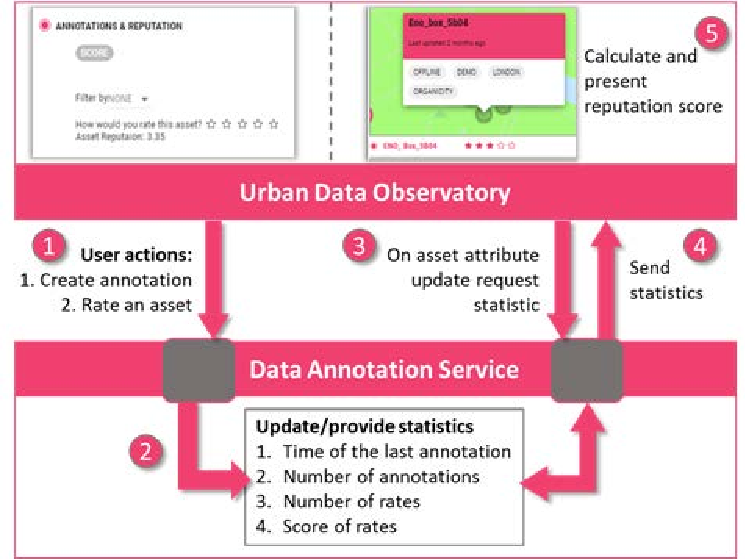
\includegraphics[scale = .65]{figures/repu1}
	\caption{Asset Reputation interface in the Urban Data Observatory (user input and calculated value)}
	\label{fig:rep}	
\end{figure}



% !TeX encoding=utf8
% !TeX spellcheck = en-US

\section{Conclusions and Future Work}
\label{sec:con}

In this work, we discussed the implementation of an EaaS framework within OrganiCity, and have presented our position regarding EaaS, i.e., to use existing IoT deployments in multiple cities in a federated manner to implement smart city prototype solutions. In this context, we presented our toolset, which enables EaaS in this application domain, in a scaled and integrated manner that has not been implemented previously. We have presented our design and implementation, discussed how OrganiCity and its toolset fit into the current smart city landscape, and presented several core components.

In order to validate this approach, we discussed learnings from deploying an EaaS framework in the wild, by running 25 experiments from independent experimenter teams. We also presented two specific experiments utilizing the OC platform as well as elaborated and discussed specific experimenter learnings, produced by using the first version of our platform. Our first findings indicate that this toolset has been utilized by the community and can be impactful. We discussed the ways in which the platform was used, where it fell short and how it has evolved through experimenter feedback. We additionally discussed results concerning the utilized architecture and scalability concerns, having used a more centralized architecture. From an architectural perspective, we can conclude that federation alternatives exist to handle potential scalability issues. In addition, following these approaches, any modification would be transparent to the systems implemented within the OC platform. We believe that this feedback, produced by such a scale of experimentation, will be very useful to the community currently working on similar aspects in the smart city domain.

OC is currently nearing its completion. The OC platform has been significantly re-factored taking experimenter learnings into account, and the updated OC platform has been put to the test in a second open call following the same approach as in the first one. Results concerning this round of experiments are not included in this article, but will be presented in our future work. 


\section*{Acknowledgment}
This work was partially supported by the OrganiCity research project funded by the European Union, under grant agreement No. 645198 of the Horizon 2020 research and innovation program. We would also like to thank the experimenter teams and volunteers who participated in OrganiCity.

\bibliographystyle{IEEEtran}
\bibliography{biblio}
\vspace{-10ex}
\begin{IEEEbiography}[{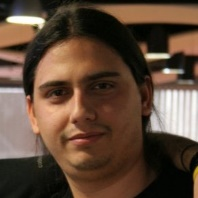
\includegraphics[width=1in,height=1in,clip,keepaspectratio]{figures/amaxilat.jpg}}]{Dimitrios Amaxilatis}
received his MSc degree in Computer Science from the University of Patras, Greece, in 2013, where he is currently pursuing the PhD degree. From 2010, he has been with the Computer Technology Institute in Patras, Greece participating in several international research projects. He was also member of the founding teams of two technological startups (codebender.cc and Sensorflare). His research interests include distributed algorithms, wireless sensor networks, home and building automation, smart city and participatory sensing.
\end{IEEEbiography}
\vspace{-7ex}
\begin{IEEEbiography}[{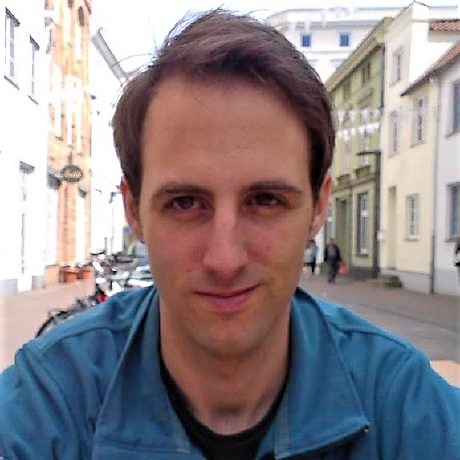
\includegraphics[width=1in,height=1in,clip,keepaspectratio]{figures/boldt.jpg}}]{Dennis Boldt}
received his MSc in Computer Science from the University of L{\"u}beck. Since 2012 he works as a research assistant at the same University and currently pursues his PhD.
He has been involved in several national and international research projects including SPITFIRE (FP7) and OrganiCity (H2020).
His research interests are peer-to-peer networks, full stack web-based technologies and network security.
\end{IEEEbiography}
\vspace{-7ex}
\begin{IEEEbiography}[{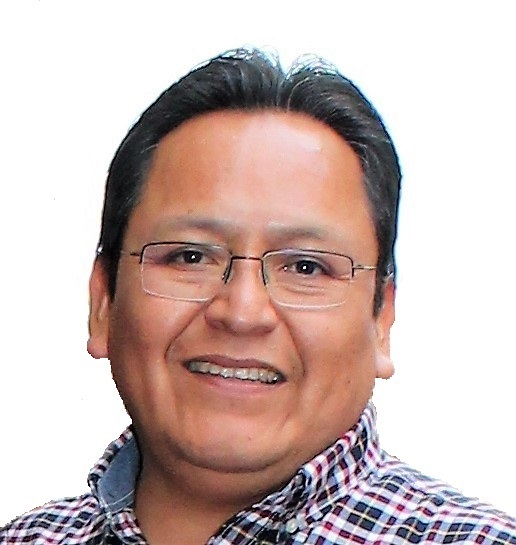
\includegraphics[width=1in,height=1in,clip,keepaspectratio]{figures/jchoque.jpg}}]{Johnny Choque}
Johnny Choque received the electronic engineering degree from the National University of Engineering, Peru, in 1995 and PhD degree (cum laude) in communications engineering from the University of Cantabria, Spain, in 2014. Since 2000, he has been employed as researcher at the University of Cantabria, working in several projects of Framework Programme and Horizon 2020 of EU. His current research interests include LPWAN, Smart Cities, IoT and Blockchain.
\end{IEEEbiography}
\vspace{-7ex}
\begin{IEEEbiography}[{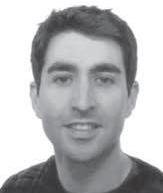
\includegraphics[width=1in,height=1in,clip,keepaspectratio]{figures/ldiez.jpg}}]{Luis Diez}
received his MSc and PhD from University of Cantabria, Spain, in 2013 and 2018 respectively. He has been involved in different international and industrial research projects. He is currently a Senior Researcher at the Network Planning and Mobile Communications Laboratory, University of Cantabria. His research interests are resource management in wireless heterogeneous networks, and IoT service provisioning.
\end{IEEEbiography}
\vspace{-7ex}
\begin{IEEEbiography}[{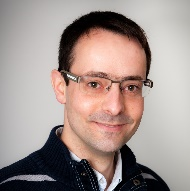
\includegraphics[width=1in,height=1in,clip,keepaspectratio]{figures/gandrille.jpg}}]{Etienne Gandrille}
received his PhD from University of Grenoble. As a researcher at Commissariat à l'\'{E}nergie atomique et aux \'{E}nergies alternatives (CEA), his research interests focus on Internet of Things, Smart Cities and Open Data. He has been involved in several international research and innovation projects including SocIoTal (FP7), OrganiCity (H2020), BigClouT (H2020) and Brain-IoT (H2020).
\end{IEEEbiography}
\vspace{-7ex}
\begin{IEEEbiography}[{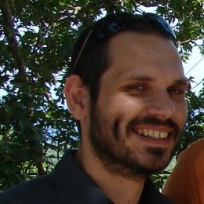
\includegraphics[width=1in,height=1in,clip,keepaspectratio]{figures/mylonasg.jpg}}]{Georgios Mylonas}
is a researcher at Computer Technology Institute and Press ''Diophantus'', Greece. He received his PhD from the University of Patras, Greece. His research interests lie in the areas of wireless sensor networks and distributed systems, IoT and pervasive games. He has been involved in the AEOLUS, WISEBED, Smartsantander, AUDIS and OrganiCity projects. He is the coordinator of the Green Awareness in Action (GAIA) H2020 project.
\end{IEEEbiography}
\vspace{-7ex}
\begin{IEEEbiography}[{
\includegraphics[width=1in,height=1in,clip,keepaspectratio]{figures/kartakis.jpg}}]
{Sokratis Kartakis} received the B.Sc. degree (Hons.) and the M.Sc. degree in computer science from the University of Crete, Heraklion, Greece, in 2006 and 2008, respectively, and the Ph.D. degree in computer science from the Department of Computing, Imperial College London, London, U.K. in 2017. He has been involved in several international research projects collaborating with Yale University, NEC Japan, and ICS-Forth Greece. Since 2017, he has been an IoT Research Scientist with Intel Labs Europe, London, U.K. His current research interests include edge signal processing and machine learning, and communication optimization for IoT.

\end{IEEEbiography}
\vspace{-7ex}
\begin{IEEEbiography}[{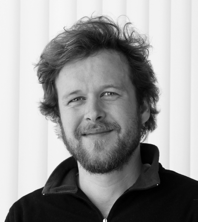
\includegraphics[width=1in,height=1in,clip,keepaspectratio]{figures/vester.jpg}}]{Lasse Steenbock Vestergaard}
received his MSc in Information Science from University of Aarhus, Denmark, and is currently pursuing a PhD focusing on IoT prototyping within Smart Cities at Alexandra Institute. He has been involved in national and international research and innovation projects including OUTSMART (FP7), SmartSantander (FP7), CityPulse (FP7), OrganiCity (H2020) and Synchronicity (H2020). His research interests are creative coding, API usability and IoT prototyping.
\end{IEEEbiography}
\end{document}